\documentclass[conference]{IEEEtran}

\usepackage[T1]{fontenc}
\usepackage[utf8]{inputenc}
\usepackage{cite}
\usepackage{amsmath,amssymb}
\usepackage{booktabs}
\usepackage{array}
\usepackage{graphicx}
\usepackage{xcolor}
\usepackage{url}
\usepackage{hyperref}
\usepackage{enumitem}
\usepackage{balance}

\hypersetup{
    colorlinks=true,
    linkcolor=black,
    citecolor=black,
    urlcolor=blue
}

\title{When Does Adaptive Retraining Help?\\
A Drift-Aware MLOps Study on Multi-Year ACS Income Data}

\author{
\IEEEauthorblockN{Taha Rasheed \quad Hamza Zahid \quad Hasnat Noor}
\IEEEauthorblockA{National University of Computers and Emerging Sciences, ISB\\
\texttt{i222009@nu.edu.pk} \quad
\texttt{i221974@nu.edu.pk} \quad
\texttt{i222049@nu.edu.pk}}
}

\begin{document}
\maketitle

\begin{abstract}
Adaptive retraining is often treated as the natural response to data drift, yet drift detection alone does not imply that newly observed labels describe a learnable replacement concept. This paper presents an end-to-end drift-aware MLOps pipeline for tabular income prediction and uses it to study when retraining helps under multi-year American Community Survey (ACS) shift. The system integrates memory-efficient ACS preprocessing, XGBoost training, statistical drift detection, policy-gated retraining, model versioning, FastAPI serving, MLflow tracking, and Prometheus/Grafana monitoring. Methodologically, the study separates three effects that are often conflated: real temporal shift, learnable covariate/feature drift, and synthetic subgroup-specific label flips. In the main 12-batch ACS experiment, immediate retraining achieves the highest mean F1 (0.7225), while a policy-gated retraining strategy improves over static deployment (0.7204 vs. 0.7155) with only 6 retraining events instead of 11. A noise-ablation study then shows why earlier retraining results appeared weak: retraining improves under clean temporal and covariate/feature drift, but degrades under label-flip stress where the new labels behave like contradictory noise. These results support a more precise conclusion: adaptive retraining is useful when drift is learnable and retraining data is stabilized, but harmful when drift simulation corrupts the target relationship. The contribution is both an operational MLOps implementation and an empirical framework for distinguishing useful adaptation from noise chasing.
\end{abstract}

\begin{IEEEkeywords}
MLOps, dataset shift, concept drift, adaptive retraining, ACS Income, XGBoost, MLflow, monitoring
\end{IEEEkeywords}

\section{Introduction}
Production machine learning systems are rarely deployed into stationary environments. Data distributions shift as populations, institutions, measurement processes, and user behavior change over time. In tabular decision systems, this problem is especially subtle: a feature distribution may drift without degrading performance, while a small change in the feature--label relationship may make yesterday's model unreliable. This distinction is central to dataset shift and concept drift research~\cite{gama2014survey,lu2019learning,webb2016characterizing}.

Modern MLOps practice responds to this risk by monitoring data and model behavior after deployment~\cite{kreuzberger2023mlops,breck2017mltest}. However, monitoring does not by itself solve adaptation. The operational question is not merely whether drift exists, but whether retraining on new data will improve future decisions. A detector can identify that a batch differs from the reference distribution; it cannot guarantee that the new batch contains a stable concept worth learning.

This paper studies that gap through a complete drift-aware MLOps pipeline for the ACS Income task derived from Folktables~\cite{ding2021retiring}. The project began as an engineering system for preprocessing data, training a model, detecting drift, retraining, serving predictions, and monitoring the deployment. During experimentation, however, a methodological issue emerged: initial synthetic concept-drift regimes based on subgroup label flips caused static and retrained models to perform similarly or made retraining worse. This raised a deeper question:

\begin{quote}
\emph{Was adaptive retraining failing because the policy was poor, or because the drift simulation asked the model to learn noise?}
\end{quote}

To answer this, we redesigned the ACS protocol around learnable temporal and covariate drift, then preserved the label-flip design as a separate stress test. The resulting study is more informative than a simple positive or negative benchmark. It shows that retraining can help, but only under the right data conditions.

The contributions of this work are:
\begin{enumerate}[leftmargin=*]
    \item a reproducible drift-aware MLOps pipeline integrating ACS preprocessing, XGBoost training, drift detection, retraining policy, model versioning, API serving, MLflow, Docker, Prometheus, and Grafana;
    \item a multi-year ACS protocol using 2016 as the baseline training year and 2017--2018 as temporally shifted evaluation data;
    \item a rolling-window retraining policy with persistent-drift gating and a stratified historical anchor;
    \item an ablation study showing that retraining improves under learnable drift but fails under subgroup label-flip noise;
    \item a practical result: policy-gated retraining recovers much of the benefit of immediate retraining while reducing retraining frequency by 45.5\%.
\end{enumerate}

\section{Related Work}
\subsection{Dataset Shift and Drift Detection}
Dataset shift occurs when the training and deployment distributions differ~\cite{quionero2009dataset}. Rabanser \emph{et al.} show that distribution testing can detect shift, but also emphasize that not every detected shift is equally harmful~\cite{rabanser2019failing}. This distinction motivates our use of both drift statistics and predictive metrics. Our detector identifies feature movement, while the policy layer decides whether a detected movement justifies retraining.

Concept drift is usually defined as change in the posterior relationship between inputs and labels over time~\cite{gama2014survey,lu2019learning}. Webb \emph{et al.} further argue for careful characterization of concept drift, because different drift types require different responses~\cite{webb2016characterizing}. Our results support that view: covariate and feature-noise drift can be useful adaptation targets, while random subgroup label flips can behave like target corruption.

\subsection{MLOps and Production ML Systems}
MLOps extends machine learning beyond offline model training into deployment, monitoring, reproducibility, and feedback loops~\cite{kreuzberger2023mlops}. Sculley \emph{et al.} describe production ML systems as sources of hidden technical debt when data dependencies, configuration, and monitoring are neglected~\cite{sculley2015debt}. Breck \emph{et al.} similarly argue that production readiness requires explicit tests and operational checks~\cite{breck2017mltest}. Our implementation reflects these concerns through configuration-driven data pipelines, Pytest coverage, versioned model artifacts, MLflow tracking, containerized services, and monitoring dashboards.

\subsection{ACS Income and XGBoost}
Folktables was introduced to move beyond the classic Adult dataset and provide richer census-derived benchmarks for fairness and robustness studies~\cite{ding2021retiring}. We use the ACS Income task because it supports large-scale multi-year experiments. The base learner is XGBoost, a strong tabular classifier with efficient tree boosting and GPU support~\cite{chen2016xgboost}. Using a strong tabular learner makes the retraining question cleaner: observed adaptation failures are less likely to be caused by an obviously weak model.

\section{System Design}
\subsection{End-to-End Pipeline}
The system is organized as a modular MLOps pipeline. It preprocesses raw data, trains a baseline model, evaluates incoming batches, detects drift, decides whether to retrain, versions updated models, and exposes both predictions and operational metrics.

\begin{figure*}[!t]
\centering
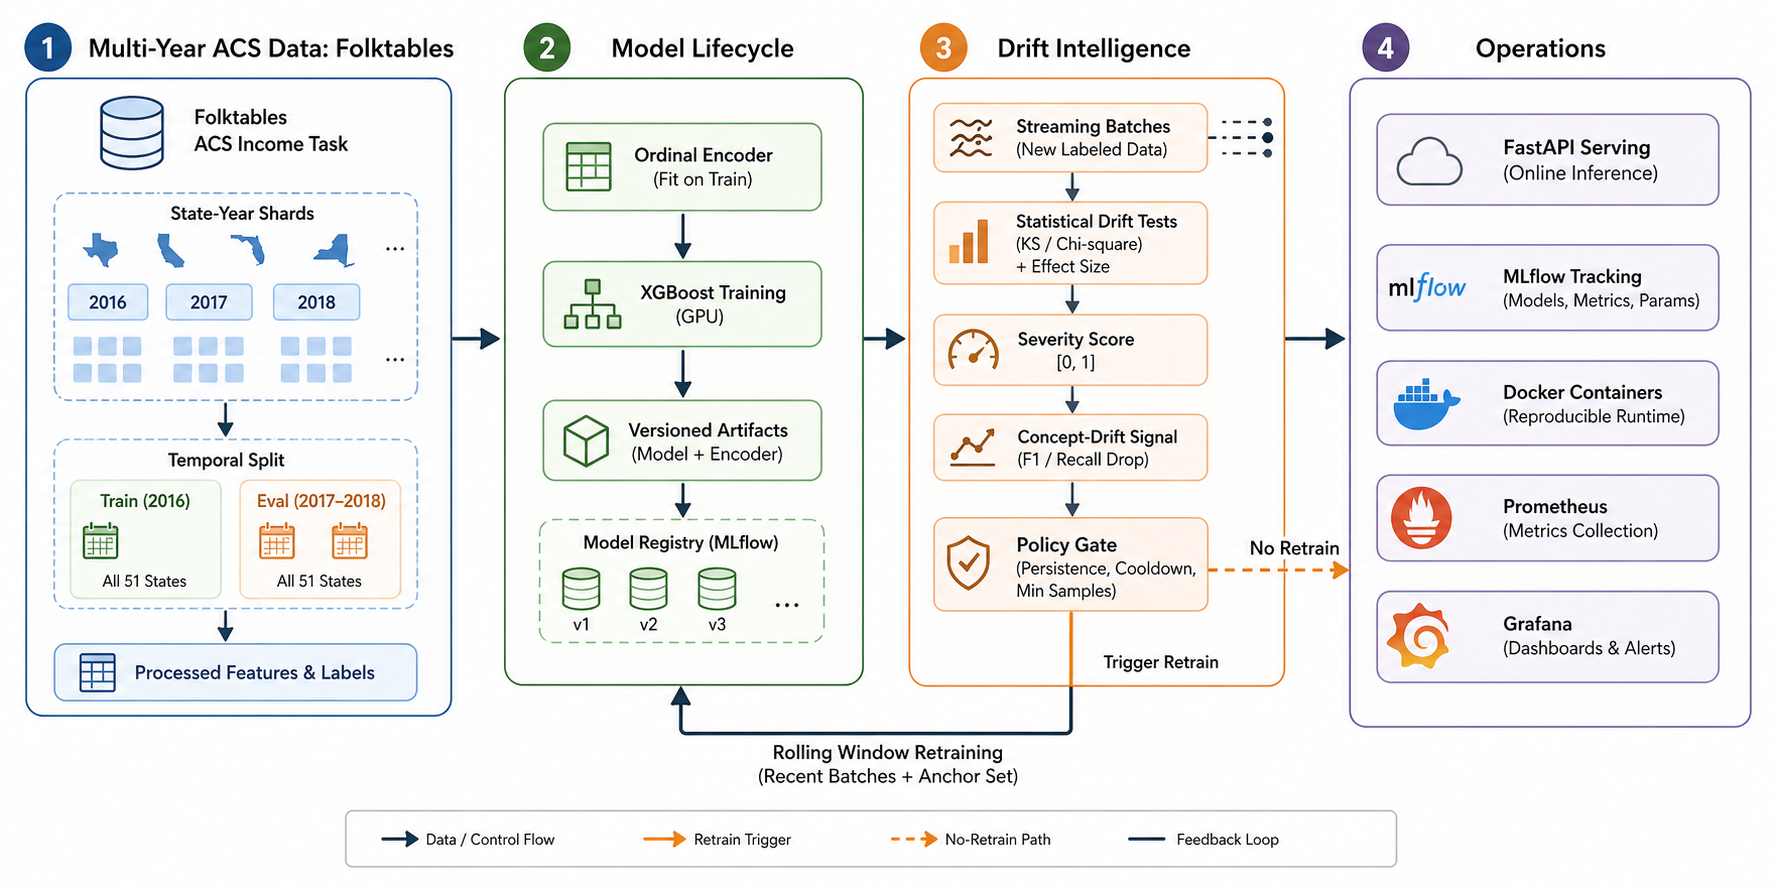
\includegraphics[width=0.95\textwidth]{figures/architecture_pipeline_i.png}
\caption{End-to-end drift-aware MLOps architecture. The pipeline separates data processing, training, drift detection, policy evaluation, retraining, serving, tracking, and observability so that modeling decisions and operational behavior can be evaluated independently.}
\label{fig:architecture}
\end{figure*}

The major components are summarized in Table~\ref{tab:stack}. The key architectural decision is that drift detection and retraining are separate modules. A batch can drift without triggering retraining if the policy gates are not satisfied.

\begin{table}[!t]
\caption{Implementation components and their roles.}
\label{tab:stack}
\centering
\begin{tabular}{p{0.27\linewidth} p{0.63\linewidth}}
\toprule
\textbf{Component} & \textbf{Role} \\
\midrule
Folktables / ACS & Multi-year income data extraction \\
XGBoost & Baseline and retrained tabular classifier \\
Drift detector & KS and chi-square feature-drift tests \\
Policy engine & Persistence, cooldown, and sample-count gates \\
MLflow & Experiment and artifact tracking \\
FastAPI & Online prediction service \\
Docker & Local service orchestration \\
Prometheus/Grafana & Metrics scraping and dashboards \\
Pytest & Regression tests for data, policy, API, and retraining \\
\bottomrule
\end{tabular}
\end{table}

\subsection{Data Processing}
The final ACS pipeline uses the 1-Year person survey for all configured U.S. states and Puerto Rico. To avoid loading the full national data into memory at once, preprocessing iterates over state-year shards, cleans each shard, attaches a \texttt{DATA\_YEAR} column, and writes processed train/test outputs. The final multi-year dataset contains 4{,}803{,}226 rows:
\begin{itemize}[leftmargin=*]
    \item 2016 training pool: 1{,}578{,}451 rows;
    \item 2017--2018 evaluation pool: 3{,}224{,}775 rows.
\end{itemize}

The prediction task is binary income classification using ten ACS Income features: age, class of worker, education, marital status, occupation, place of birth, relationship, weekly work hours, sex, and race.

\section{Methodology}
\subsection{Drift Detection}
For each incoming batch, numerical features are compared with the reference distribution using Kolmogorov--Smirnov tests, and categorical features are compared using chi-square tests. Multiple testing correction and minimum effect-size thresholds are used to reduce false alarms in large samples. A batch-level severity score summarizes the proportion and magnitude of drifted features.

\subsection{Retraining Policy}
The policy engine evaluates four conditions before retraining:
\begin{enumerate}[leftmargin=*]
    \item drift severity exceeds a configurable threshold;
    \item enough new labeled samples have accumulated;
    \item cooldown since the previous retrain has elapsed;
    \item the drift signal persists across consecutive batches.
\end{enumerate}

Retraining data is selected with a bounded rolling window of recent labeled batches plus a 10\% stratified anchor sample from the original training year. The anchor is intentionally retained because the ablation study shows that pure sliding-window retraining is unstable at the current batch size.

\subsection{Experiment Design}
The final study has three parts.

\textbf{Main learnable-drift experiment.} The main ACS drift configuration avoids synthetic label flips. It uses temporal batch sourcing, covariate shifts, categorical redistribution, and feature-noise perturbations. This is the primary experiment used to evaluate static, immediate, and policy-gated retraining.

\textbf{Noise-ablation experiment.} The earlier subgroup label-flip design is retained only as a stress test. Four streams are compared: clean temporal batches, covariate/feature shift, label-flip-only stress, and mixed drift with label flips.

\textbf{Temporal regime diagnostic.} Additional models are trained on 2016-only, 2017--2018-only, 2017--2018 plus a 10\% 2016 anchor, and a 2016--2018 expanding window. All are evaluated on held-out 2018 data to determine whether later-year ACS data contains learnable signal.

\section{Results}
\subsection{Main ACS Retraining Experiment}
Table~\ref{tab:main_results} summarizes the final 12-batch learnable-drift ACS experiment. Static deployment achieves mean F1 of 0.7155. Immediate retraining improves mean F1 to 0.7225 but retrains after 11 of 12 batches. Policy-gated retraining achieves mean F1 of 0.7204 with only 6 retraining events.

\begin{table}[!t]
\caption{Main ACS learnable-drift results.}
\label{tab:main_results}
\centering
\begin{tabular}{lcccc}
\toprule
\textbf{Policy} & \textbf{Mean Acc.} & \textbf{Mean F1} & \textbf{F1 Deg. Area} & \textbf{Retrains} \\
\midrule
Static & 0.7667 & 0.7155 & 0.4246 & 0 \\
Immediate & 0.7873 & 0.7225 & 0.3365 & 11 \\
Policy-Standard & 0.7837 & 0.7204 & 0.3604 & 6 \\
\bottomrule
\end{tabular}
\end{table}

\begin{figure*}[!t]
\centering
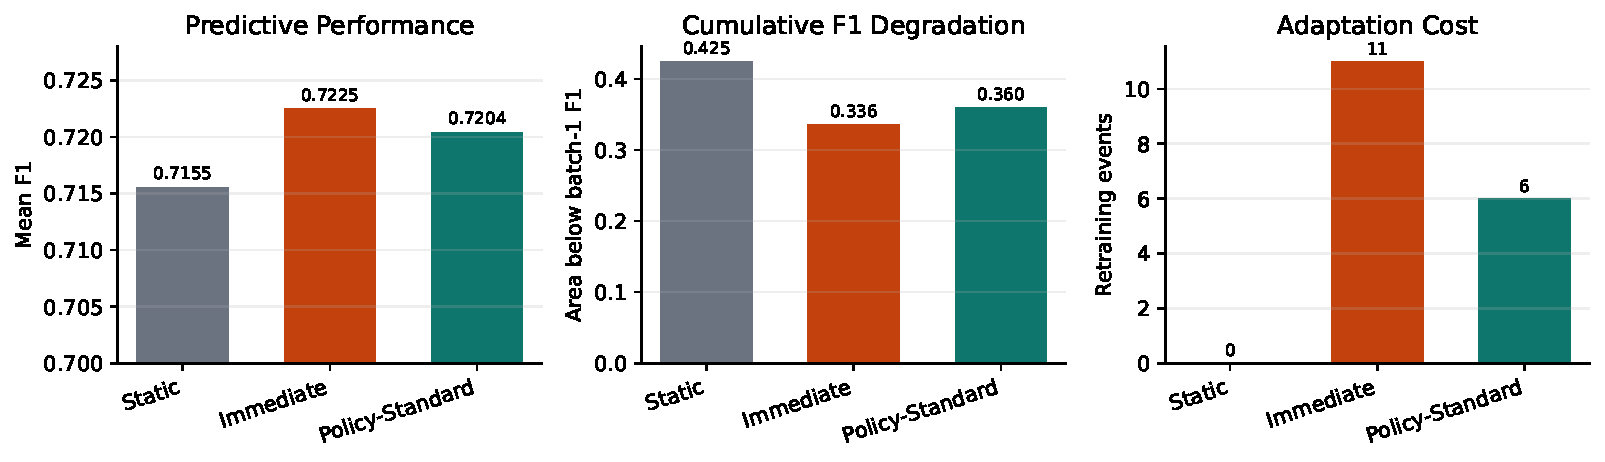
\includegraphics[width=0.95\textwidth]{figures/main_policy_tradeoff.pdf}
\caption{Main ACS policy trade-off. Immediate retraining gives the highest mean F1 and lowest cumulative degradation, but policy-gated retraining captures most of the gain while cutting retraining events from 11 to 6.}
\label{fig:main_tradeoff}
\end{figure*}

The result is promising for two reasons. First, after removing unrealistic label flips from the main experiment, adaptive retraining now improves over static deployment. Second, the policy engine reduces adaptation cost substantially relative to immediate retraining. Policy-Standard closes approximately 70\% of the mean-F1 gap between Static and Immediate while using 45.5\% fewer retraining events.

The result is not a blanket victory for retraining. Immediate retraining still has the best mean F1, and the next-batch recovery metric remains noisy because later batches are often harder than the retraining-trigger batch. Nevertheless, the core pattern changed: under learnable drift, retraining is beneficial.

\subsection{Noise-Ablation Study}
The ablation study explains why earlier experiments showed little benefit from retraining. Table~\ref{tab:ablation} compares static deployment, anchored policy retraining, and pure sliding-window retraining across four stream designs.

\begin{table*}[!t]
\caption{Noise-ablation results: mean F1 by drift type and strategy.}
\label{tab:ablation}
\centering
\begin{tabular}{lccc}
\toprule
\textbf{Stream} & \textbf{Static} & \textbf{Policy + Anchor} & \textbf{Policy Sliding, No Anchor} \\
\midrule
Clean temporal & 0.7248 & \textbf{0.7274} & 0.7180 \\
Covariate/feature shift & 0.7155 & \textbf{0.7236} & 0.7054 \\
Label-flip only & \textbf{0.6906} & 0.6874 & 0.6817 \\
Mixed with label flips & \textbf{0.6678} & 0.6651 & 0.6432 \\
\bottomrule
\end{tabular}
\end{table*}

\begin{figure*}[!t]
\centering
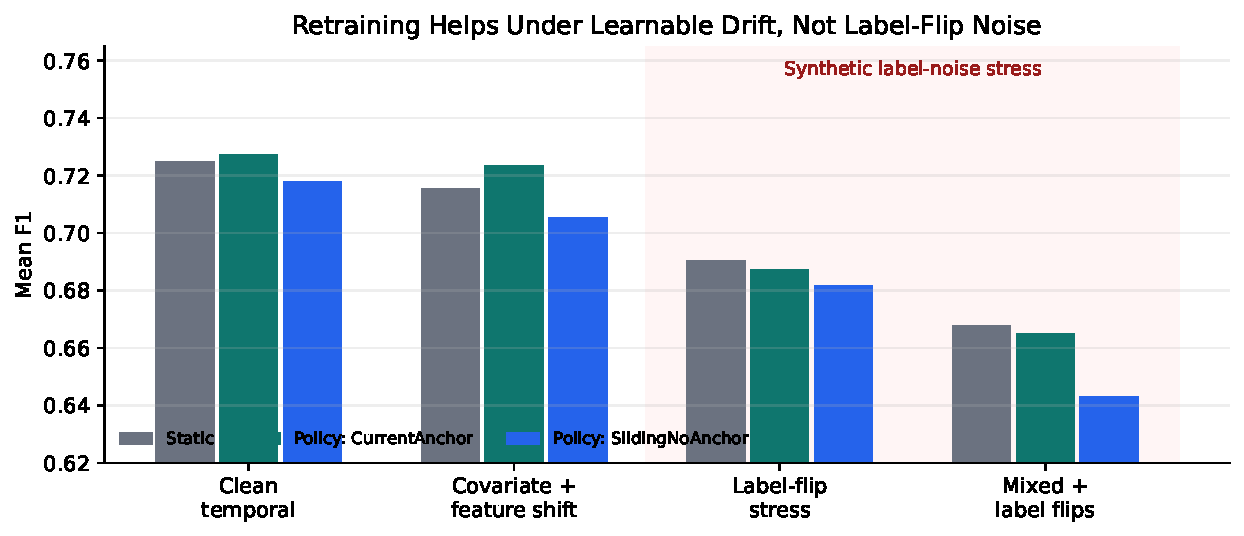
\includegraphics[width=0.88\textwidth]{figures/noise_ablation_summary.pdf}
\caption{Noise-ablation summary. Retraining improves under clean temporal and covariate/feature drift, but degrades under label-flip stress. This shows that subgroup-specific label flips behave more like contradictory label noise than a stable concept drift target.}
\label{fig:noise_ablation}
\end{figure*}

This is the central empirical insight of the paper. Retraining is not inherently ineffective; rather, it is sensitive to whether the new labels represent a learnable regime. Under clean temporal drift, the anchored policy improves mean F1 by 0.0026 over static. Under covariate/feature drift, the improvement grows to 0.0081. Under label-flip-only stress, however, retraining loses to static, and the pure sliding-window policy performs worst. The same pattern appears under mixed label-flip stress.

The ablation also clarifies the role of the historical anchor. A pure sliding window might seem theoretically appropriate for drift, but at the current batch size it is too small and noisy. The 10\% anchor acts as regularization and improves stability.

\subsection{Temporal Regime Diagnostic}
The temporal diagnostic tests whether later-year ACS data contains a learnable rule shift. Table~\ref{tab:regime} and Fig.~\ref{fig:regime} show that training on 2017--2018 improves held-out 2018 F1 from 0.7160 to 0.7399. Adding a 10\% 2016 anchor is essentially tied at 0.7400, while the full expanding window is slightly lower at 0.7378.

\begin{table}[!t]
\caption{Training-regime diagnostic on held-out 2018 data.}
\label{tab:regime}
\centering
\begin{tabular}{lcc}
\toprule
\textbf{Training regime} & \textbf{Accuracy} & \textbf{F1} \\
\midrule
2016 only & 0.7790 & 0.7160 \\
2017--2018 only & 0.8111 & 0.7399 \\
2017--2018 + 10\% 2016 anchor & 0.8112 & 0.7400 \\
2016--2018 expanding & 0.8111 & 0.7378 \\
\bottomrule
\end{tabular}
\end{table}

\begin{figure*}[!t]
\centering
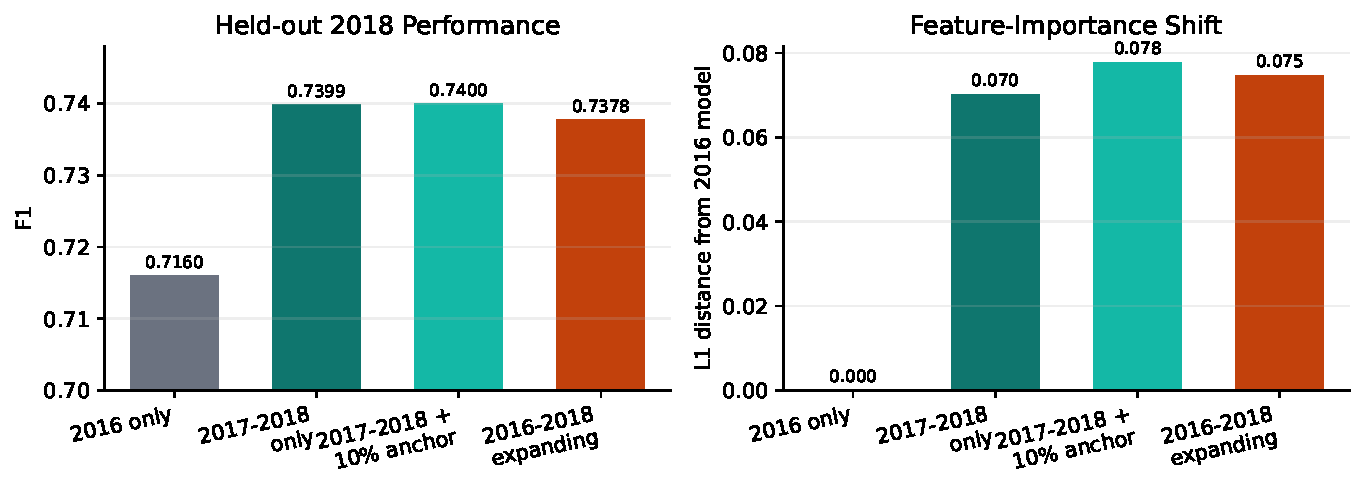
\includegraphics[width=0.88\textwidth]{figures/temporal_regime_diagnostics.pdf}
\caption{Temporal regime diagnostic. Later-year ACS data improves held-out 2018 F1, while feature-importance distances from the 2016 model remain modest. The shift is learnable but not a complete rule reversal.}
\label{fig:regime}
\end{figure*}

Feature-importance diagnostics show modest but nonzero change from the 2016 model. The top feature remains education (\texttt{SCHL}) in every regime, so the temporal change is not a wholesale reversal of the decision function. It is better interpreted as a learnable distributional and weighting shift.

\section{Discussion}
\subsection{Why the Original Experiment Looked Flat}
The original retraining results were weak because the experiment mixed learnable drift with subgroup label flips. A label flip changes the target for selected rows without creating a stable new structural relationship. From the learner's perspective, this can be target noise. A retrained model then tries to fit contradictions, while a static model avoids chasing them. The ablation confirms this interpretation: static deployment wins exactly in the label-flip regimes.

\subsection{What the Final Results Mean}
The final results support a conditional view of adaptive retraining:
\begin{itemize}[leftmargin=*]
    \item drift detection is necessary but not sufficient;
    \item retraining helps when incoming labeled data reflects a stable new regime;
    \item retraining can hurt when labels are noisy or contradictory;
    \item at small online batch sizes, a historical anchor can stabilize retraining;
    \item policy gating provides a practical cost-performance compromise.
\end{itemize}

This is stronger than simply reporting that retraining improves. It identifies the boundary condition under which retraining is useful.

\subsection{Operational Implications}
From an MLOps perspective, the study recommends separating drift monitoring from retraining decisions. A production system should log detected drift, measure labeled performance degradation, and apply policy gates before retraining. It should also evaluate retraining with recovery and degradation metrics rather than only aggregate accuracy.

The system also demonstrates why tooling matters. MLflow records model versions and metrics; Docker makes the serving stack reproducible; Prometheus and Grafana expose operational behavior; and tests protect policy logic from accidental regression. These tools do not make the model better directly, but they make adaptation decisions inspectable and reproducible.

\section{Threats to Validity}
The study has several limitations. First, part of the drift remains simulated, even though the base stream is multi-year ACS. Second, only XGBoost is evaluated; neural tabular models or online learners could respond differently. Third, retraining assumes labeled feedback is available for each batch, which may be delayed in real deployments. Fourth, the optimal anchor size likely depends on batch size and drift intensity. Finally, ACS Income is a structured benchmark, not a live production system.

\section{Conclusion}
This paper presented a drift-aware MLOps pipeline and used it to answer a practical question: when does adaptive retraining help? The final evidence is clear. On the main learnable ACS drift experiment, retraining improves over static deployment, and policy-gated retraining achieves most of the immediate-retraining benefit with far fewer retraining events. On label-flip stress tests, retraining degrades performance, showing that synthetic subgroup label flips behave more like target noise than meaningful concept drift.

The broader lesson is that adaptive retraining should not be triggered merely because data changed. It should be triggered when the new data is sufficiently clean, persistent, and learnable. The pipeline developed here provides an operational and experimental framework for making that distinction.

\balance
\bibliographystyle{IEEEtran}
\bibliography{references}

\end{document}
